% Comandos especiais



% COMANDO \matriz %%%%%%%%%%%%%%%%%%%%%%%%%%%%%%%%%%%%%%%%%%%%%%%%%%%%
\newcommand{\matriz}[1]{%
  \begin{equation}\begin{bmatrix}
    #1
  \end{bmatrix}\end{equation}
}


% COMANDO \grafico %%%%%%%%%%%%%%%%%%%%%%%%%%%%%%%%%%%%%%%%%%%%%%%%%%
\newcommand{\grafico}{%
  \begin{center}
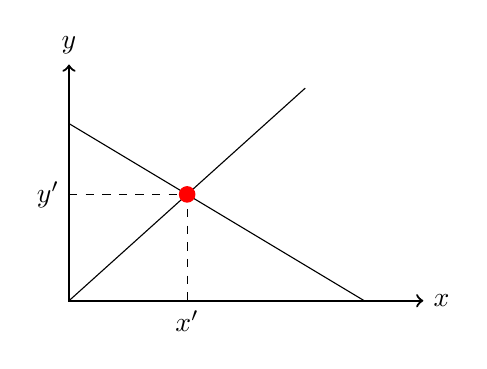
\begin{tikzpicture}[scale=1.5]
    % Draw axes
    \draw [<->,thick] (0,2) node (yaxis) [above] {$y$}
        |- (3,0) node (xaxis) [right] {$x$};
    % Draw two intersecting lines
    \draw (0,0) coordinate (a_1) -- (2,1.8) coordinate (a_2);
    \draw (0,1.5) coordinate (b_1) -- (2.5,0) coordinate (b_2);
    % Calculate the intersection of the lines a_1 -- a_2 and b_1 -- b_2
    % and store the coordinate in c.
    \coordinate (c) at (intersection of a_1--a_2 and b_1--b_2);
    % Draw lines indicating intersection with y and x axis. Here we use
    % the perpendicular coordinate system
    \draw[dashed] (yaxis |- c) node[left] {$y'$}
        -| (xaxis -| c) node[below] {$x'$};
    % Draw a dot to indicate intersection point
    \fill[red] (c) circle (2pt);
\end{tikzpicture}
\end{center}
}



% COMANDO \funcao{X} %%%%%%%%%%%%%%%%%%%%%%%%%%%%%%%%%%%%%%%%%%%%%%%%%%%
\newcommand{\funcao}[1]{%

%\begin{equation}
%f(x) = \frac{#1}{#2} \mathrm e^x
%\end{equation}

\begin{center}
\begin{tikzpicture}[domain=0:4]
    \draw[very thin,color=gray] (-0.1,-1.1) grid (3.9,3.9);
    \draw[->] (-0.2,0) -- (4.2,0) node[right] {$x$};
    \draw[->] (0,-1.2) -- (0,4.2) node[above] {$f(x)$};
    \draw[color=red] plot[id=x] function{x} 
        node[right] {$f(x) =x$};
    \draw[color=blue] plot[id=sin] function{sin(x)} 
        node[right] {$f(x) = \sin x$};
    \draw[color=orange] plot[id=exp] function{ #1*exp(x)} 
        node[right] {$f(x) = {#1} \mathrm e^x$};
\end{tikzpicture}
\end{center}
}


% COMANDO \efeito{}

\newcommand{\efeito}[1]{%
	\begin{center}
	\begin{tikzpicture}
		\draw [help lines] (0,0) grid (4,4);
		\foreach \i in {0,0.1,...,2}
		\fill ($(2,2) !\i! \i*#1:(3,2)$) circle (2pt);
	\end{tikzpicture}

	$#1$ (tente adivinhar o que este núumero faz)
	\end{center}
}


% =========================================================================
% Conteúdo %%%%%%%%%%%%%%%%%%%%%%%%%%%%%%%%%%%%%%%%%%%%%%%%%%%%%%%%%%%%%%%%


\newcommand\titulo{A volta dos que não foram}
\newcommand\autor{Alunos da quarta série C}

% Equipe
\newcommand\organizador{José Menino}
\newcommand\editor{Jorge Sallum}
\newcommand\capista{Ronaldo Moreno}
\newcommand\revisor{Pedro Silvestre}

% Escola
\newcommand\escola{Rainha da Paz}
\newcommand\telefoneescola{23123123123}
\newcommand\escolaendereco{Rua Duarte da Costa 909,\\ Cotia-SP\\Brasil}
\newcommand{\urlescola}{www.escola.com.br}
\newcommand{\logoescola}{Logo_capes.jpg}

% Dados bibliográficos
\newcommand\ccdA{Literatura infanto-juvenil}
\newcommand\ccdB{Ficção contemporânea}
\newcommand\cidade{São Paulo}
\newcommand\ano{2013}
\newcommand\direitos{Hedra}
\newcommand\isbn{Não cadastrado}

% Conteúdo do livro
\newcommand\introducao{\chapter{Introdução}
                          \grafico{}
                          \lipsum[1-4]
			\begin{figure}
			  \funcao{0.1}
			\end{figure}
			  \lipsum[5-6]}
\newcommand\texto{\chapter{Texto 1}
    \matriz{12 & 12 & 12\\ 
    34 & 2 & 12\\
    12 & 12 & 12\\}
                          \lipsum[2]
    \matriz{2 & 22 \\
            34 & 34}
                  \chapter{Texto 2}
			  \efeito{200}
                          \lipsum[42-53]}


